%%=============================================================================
%% Voorwoord
%%=============================================================================

\chapter*{Bijlage}%
\label{ch:bijlage}

\section{Berekenen van de R0 waarden}
\label{lst:kalibratie}
\begin{lstlisting}[language=Java, caption={Berekenen van de R0 waarden}]
float R0_berekenen(float analogeWaarde, float luchtconstante) {
    float Rs;
    float R0;
    float V_out;
    float V_cc = 5.0;
    float maxAnaloog = 1023.0;
    float R_l = 1.0;
    
    //waarde omzetten naar spanning
    V_out = (analogeWaarde*V_cc)/maxAnaloog;
    
    //Rs berekenen
    Rs = ((V_cc*R_l)/V_out)-R_l;
    
    //R0 berekenen met luchtconstante
    R0 = Rs/luchtconstante;
    
    return R0;
}
\end{lstlisting}


\section{Berekenen van de ppm waarden voor de MQ-135}
\label{lst:ppm_mq135}
\begin{lstlisting}[language=Java, caption={Berekenen van de ppm waarden voor de MQ-135}]
// ppm meten MQ-135

//R0 berekent met kalibratie script
float R0_MQ135 = 9.59;

float Rs_MQ135;

//pin vd sensor 
int MQ135 = A1;

float analogeWaarde_MQ135;

float MQ135_CO_ppm;
float MQ135_NH4_ppm;
float MQ135_CO2_ppm;
float MQ135_alcohol_ppm;
float MQ135_tolueen_ppm;
float MQ135_aceton_ppm;

//waarden van grafieken (x1, y1, x2, y2)
float MQ135_CO2[4] = {10.72, 2.78, 191.15, 1.35};
float MQ135_NH4[4] = {10.61, 2.49, 190.20, 0.77};
float MQ135_CO[4] = {10.72, 2.24, 188.31, 0.81};
float MQ135_alcohol[4] = {10.51, 1.86, 189.25, 0.74};
float MQ135_tolueen[4] = {10.45, 1.52, 188.31, 0.65};
float MQ135_aceton[4] = {10.72, 1.39, 189.25, 0.59};


void setup() {
    Serial.begin(9600);
}

void loop() {
    analogeWaarde_MQ135 = analogRead(MQ135);
    
    Rs_MQ135 = Rs_berekenen(analogeWaarde_MQ135);
    
    MQ135_CO_ppm = ppm_berekenen(R0_MQ135, Rs_MQ135, MQ135_CO);
    MQ135_NH4_ppm = ppm_berekenen(R0_MQ135, Rs_MQ135, MQ135_NH4);
    MQ135_CO2_ppm = ppm_berekenen(R0_MQ135, Rs_MQ135, MQ135_CO2);
    MQ135_alcohol_ppm = ppm_berekenen(R0_MQ135, Rs_MQ135, MQ135_alcohol);
    MQ135_tolueen_ppm = ppm_berekenen(R0_MQ135, Rs_MQ135, MQ135_tolueen);
    MQ135_aceton_ppm = ppm_berekenen(R0_MQ135, Rs_MQ135, MQ135_aceton);
    
    Serial.print("MQ135_CO_ppm = ");
    Serial.println(MQ135_CO_ppm);
    
    Serial.print("MQ135_NH4_ppm = ");
    Serial.println(MQ135_NH4_ppm);
    
    Serial.print("MQ135_CO2_ppm = ");
    Serial.println(MQ135_CO2_ppm);
    
    Serial.print("MQ135_alcohol_ppm = ");
    Serial.println(MQ135_alcohol_ppm);
    
    Serial.print("MQ135_tolueen_ppm = ");
    Serial.println(MQ135_tolueen_ppm);
    
    Serial.print("MQ135_aceton_ppm = ");
    Serial.println(MQ135_aceton_ppm);
    
    delay(5000);
}


float Rs_berekenen(float analogeWaarde) {
    float Rs;
    float V_out;
    float V_cc = 5.0;
    float maxAnaloog = 1023.0;
    float R_l = 1.0;
    
    //waarde omzetten naar spanning
    V_out = (analogeWaarde*V_cc)/maxAnaloog;
    
    //Rs berekenen
    Rs = ((V_cc*R_l)/V_out)-R_l;
    
    return Rs;
}

float ppm_berekenen(float R0, float Rs, float waarden[4]) {
    float b;
    float m;
    float ppm;
    
    m = (log10(waarden[3])-log10(waarden[1]))/(log10(waarden[2])-log10(waarden[0]));
    b = log10(waarden[1]) - m*log10(waarden[0]);
    
    ppm = pow((Rs/(R0*pow(10, b))),(1/m));
    
    return ppm;
}
    
\end{lstlisting}



\section{Het initialiseren van de ESP01 WiFi module}
\label{sec:esp_init}

\subsection{Downloaden van de firmware}
\label{subsec:firmware}

Figuur 
~\ref{fig:esp_circuit} toont aan hoe de ESP01 moet worden aangesloten om de firmware te kunnen downloaden.

\begin{figure}[h]
    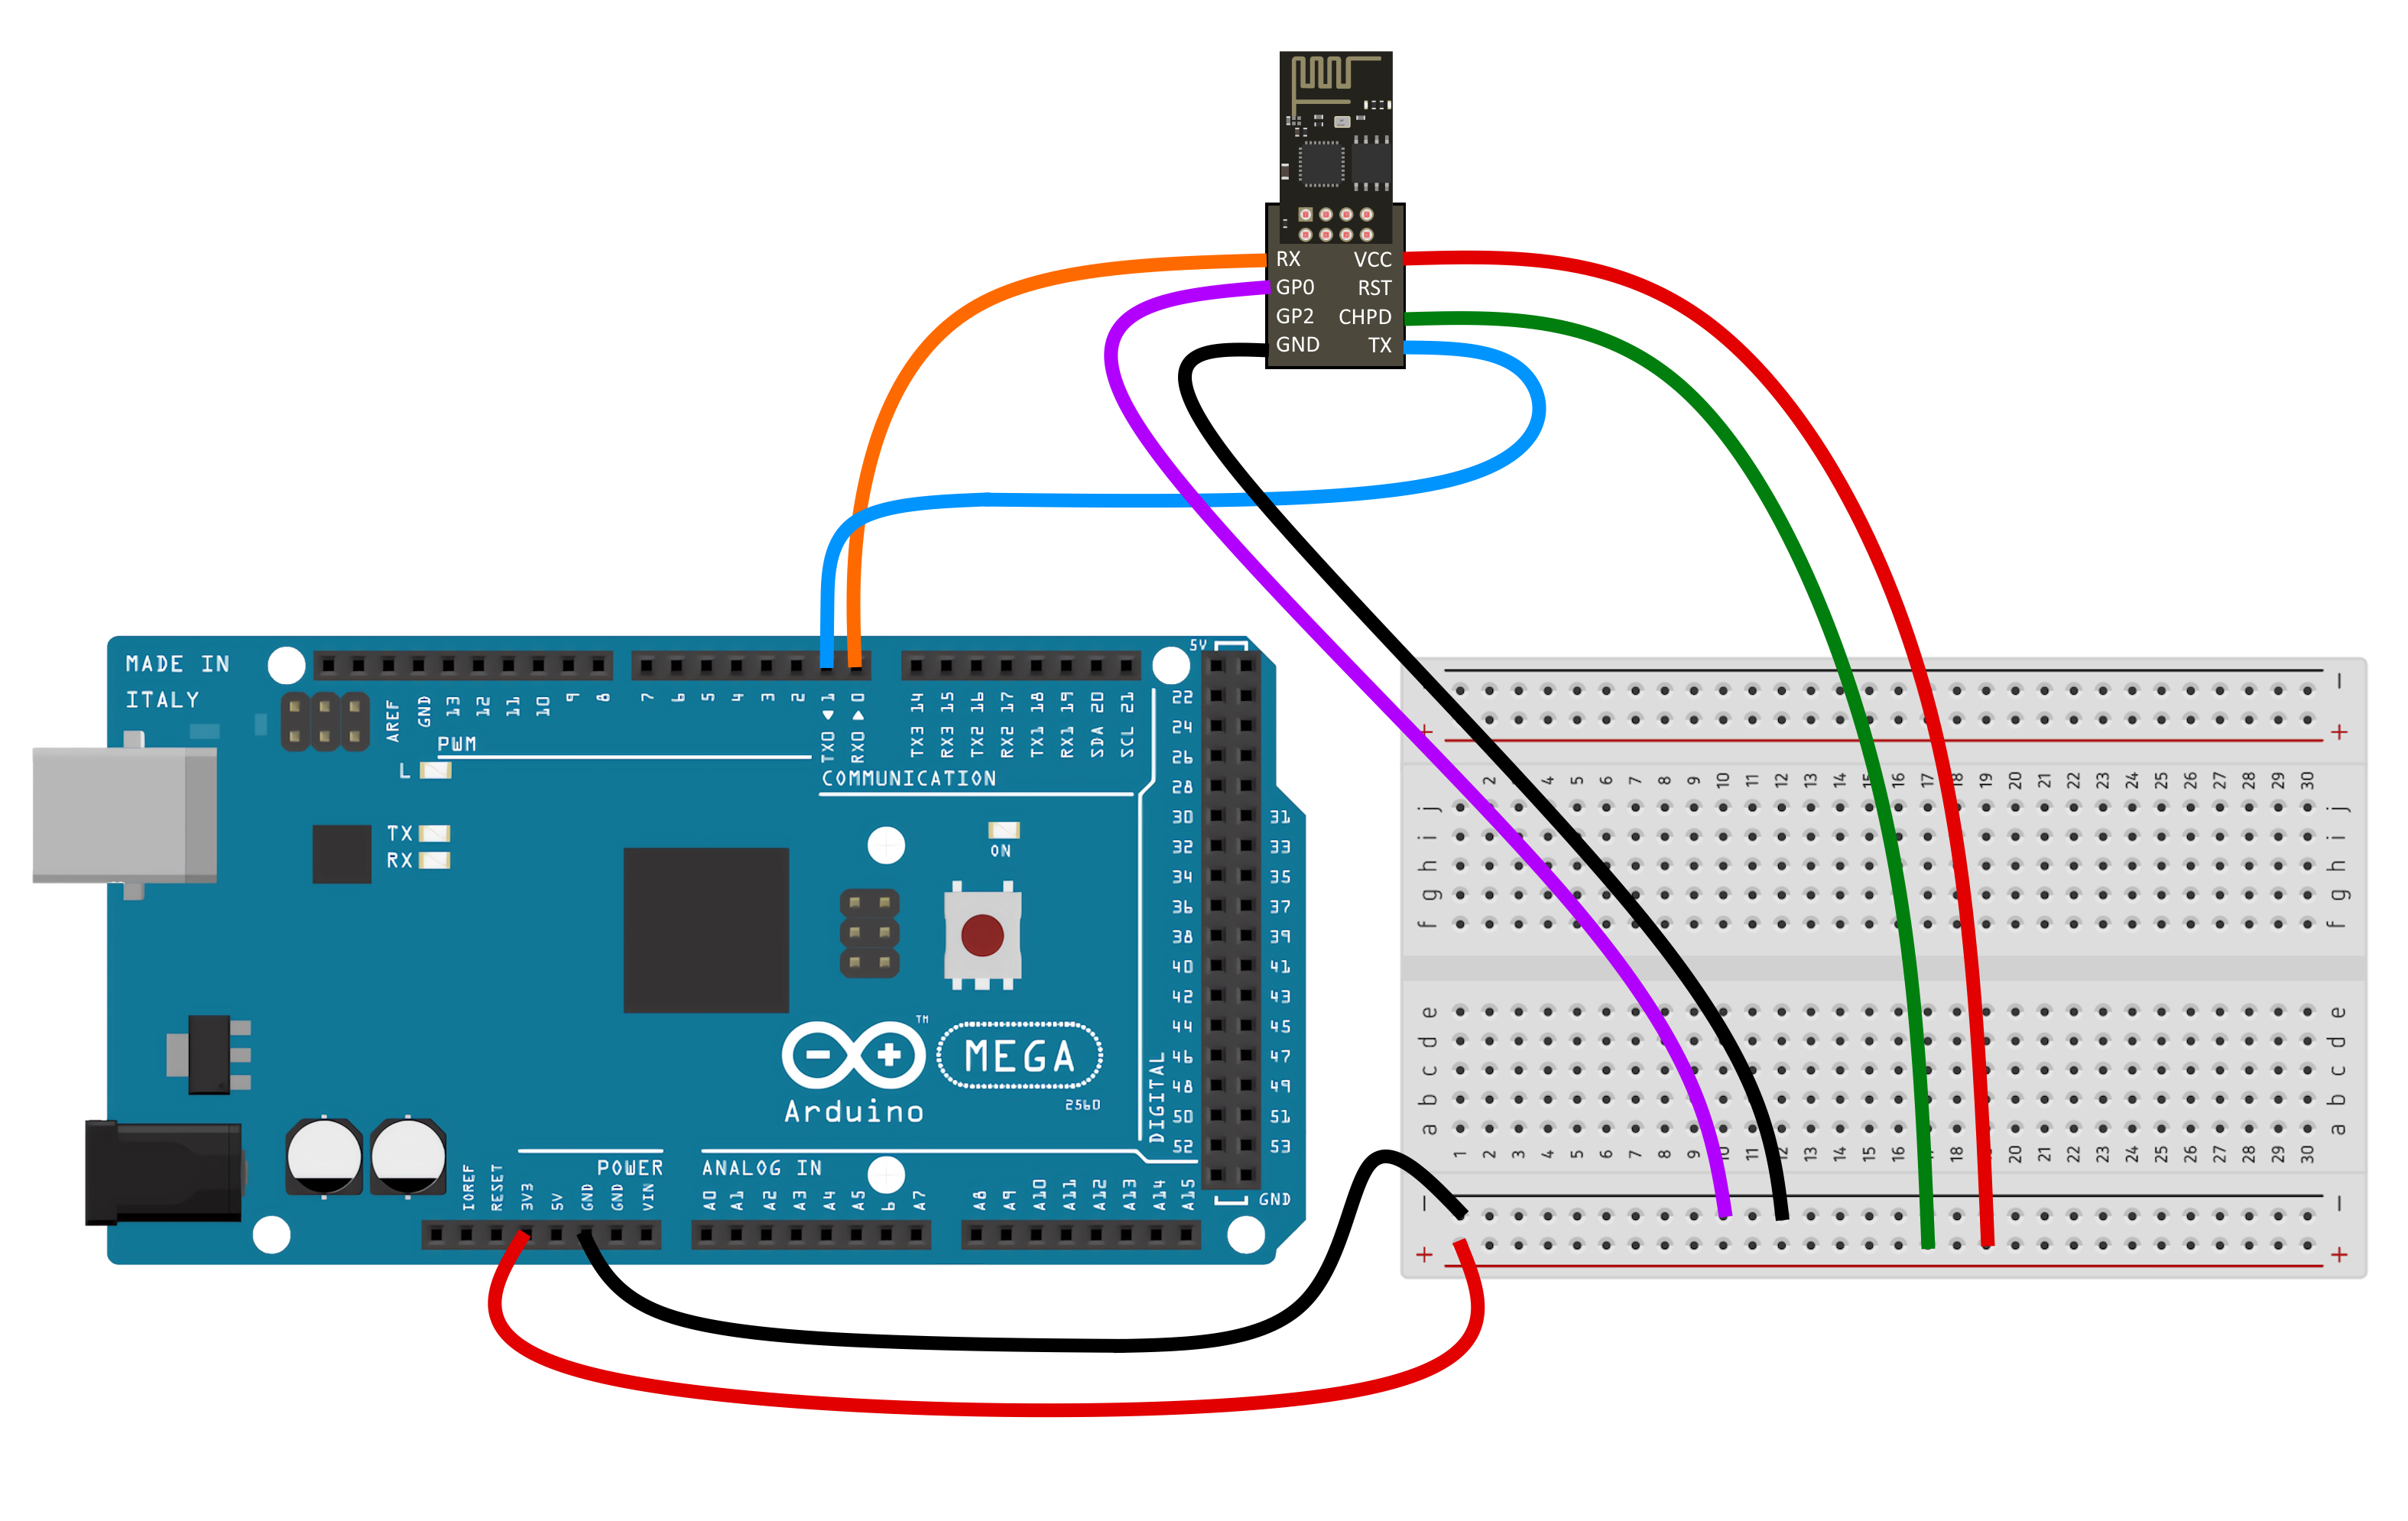
\includegraphics[scale=0.2, center]{esp_circuit.png}
    \caption[Circuit ESP01]{Circuit voor het instellen van de ESP01}
    \label{fig:esp_circuit}
\end{figure}

De juiste flasher software is te vinden in \href{https://drive.google.com/open?id=1tD7IpE4rPMOWyQHP6xzjdRKjJAyeEZPj}{deze} deze Google drive. De juiste firmware is \href{https://wiki.aprbrother.com/en/Firmware_For_ESP8266.html}{hier} te vinden, de correcte versie is v0.9.5.2.

Vervolgens kan de juiste firmware worden geüpload door de juiste poort van de Arduino te selecteren en te beginnen met downloaden. Tijdens het downloaden is het belangrijk dat er geen Serial monitors open staan in de Arduino IDE.



\subsection{Instellen van de ESP01}
\label{subsec:instellen}

Nadat de juiste firmware is geïnstalleerd op de ESP01 kan deze worden bereikt met de command-line-interface in de Arduino IDE. Vooraleer er AT-commando's kunnen worden verstuurd moet er een lege applicatie worden geüpload op de Arduino. Hierna kan de ESP bereikt worden, een kleine test is het commando AT, waarop OK moet worden geantwoord:

\begin{lstlisting}[language=Java,caption={Test of de ESP01 bereikbaar is}]
AT

OK
\end{lstlisting}

Vervolgens moeten de volgende commando's worden verstuurd:
\begin{lstlisting}[language=Java,caption={ESP01 voorbereiden}]
AT+CIOBAUD=9600 //baud rate veranderen naar 9600

AT+CWMODE=1     //WiFi modus correct instellen

AT+CWJAP="netwerknaam","paswoord"   //ESP01 verbinden met WiFi netwerk

AT+CIPMUX=0     //enkele verbinding inschakelen    
\end{lstlisting}


\section{Visualisatie in Thingspeak via Matlab}
\label{sec:matlab}

\begin{lstlisting}[language=Matlab,caption={Visualisatie in matlab}]
readChannelID = CHANNEL_ID;
readAPIKey = 'READ_API_KEY';

fieldIDs = [1, 2, 3, 4, 5, 6, 7, 8];

% aantal datapunten die worden getoont
numPoints = 10;

% data lezen van Thingspeak
data = thingSpeakRead(readChannelID, 'Fields', fieldIDs, 'NumPoints', numPoints, 'ReadKey', readAPIKey);

% per veld de data selecteren
MQ135_CO2_ppm = data(:, 1);
MQ135_NH4_ppm = data(:, 2);
MQ7_CO_ppm = data(:, 3);
MQ4_CH4_ppm = data(:, 4);
MQ7_H2_ppm = data(:, 5);
MQ4_LPG_ppm = data(:, 6);
Temperature = data(:, 7);
Luchtvochtigheid = data(:, 8);


figure;

subplot(2, 4, 1);
plot(MQ135_CO2_ppm);
title('MQ135 CO2');

subplot(2, 4, 2);
plot(MQ135_NH4_ppm);
title('MQ135 NH4');

subplot(2, 4, 3);
plot(MQ7_CO_ppm);
title('MQ7 CO');

subplot(2, 4, 4);
plot(MQ4_CH4_ppm);
title('MQ4 CH4');

subplot(2, 4, 5);
plot(MQ7_H2_ppm);
title('MQ7 H2');

subplot(2, 4, 6);
plot(MQ4_LPG_ppm);
title('MQ4 LPG');

subplot(2, 4, 7);
plot(Temperature);
title('Temperatuur');

subplot(2, 4, 8);
plot(Luchtvochtigheid);
title('Luchtvochtigheid');

\end{lstlisting}


\section{Instellen van de database}
\label{sec:database}

De databank werd gehost via Apache, dit gebeurde met de hulp van XAMPP. XAMPP is een open source applicatie gemaakt door ApacheFriends. Deze omgeving biedt verschillende diensten aan, zoals de Apache-webserver en MySQL. Via het controle paneel kan Apache worden opgestart waarna deze draait op poort 80. Het is belangrijk dat er in de firewall configuratie van de computer een uitzondering wordt gemaakt voor \verb|C:\xampp\apache\bin\httd.exe|, anders zal Apache worden geblokkeerd.

\begin{figure}[h]
    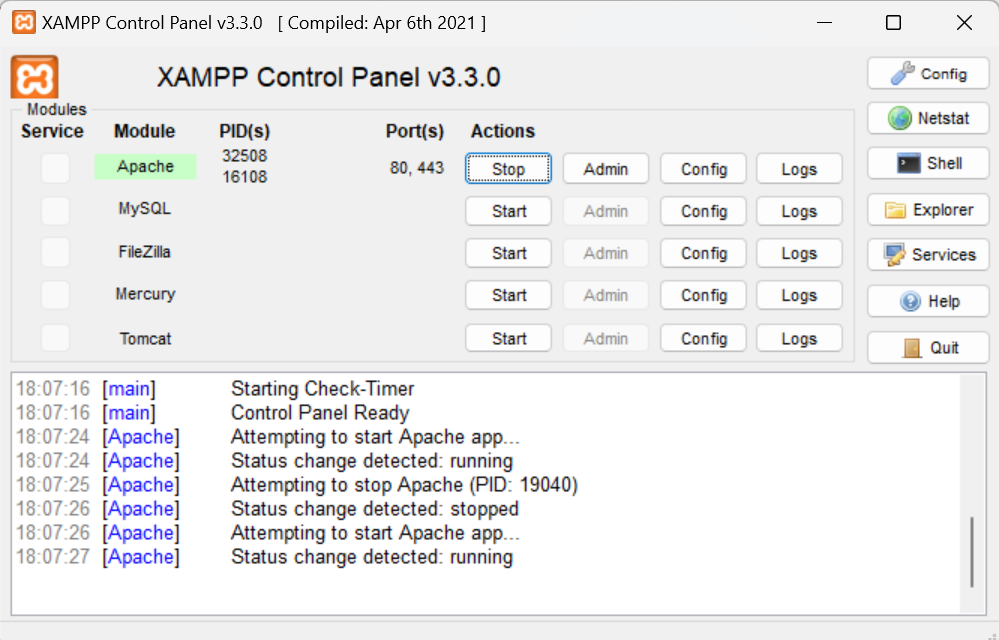
\includegraphics[scale=0.5, center]{XAMPP.png}
    \caption[XAMPP controlepaneel]{Controlepaneel van XAMPP}
    \label{fig:XAMPP}
\end{figure}

Vervolgens moeten de PHP-files worden geschreven, tenslotte moeten deze in de folder \verb|C:\xampp\htdocs| worden gezet staan zodat Apache deze kan vinden.

\section{Finale code}
\label{sec:finale_code}

\subsection{Berekenen van de R\textsubscript{0} waardes}
\label{subsec:script_R0}

\begin{lstlisting}[language=Java,caption={Berekenen en verzenden van de R0 waardes}]
// Kalibratie MQ-4, MQ-135 en MQ-7
// te doen in schone buitenlucht na opwarmperiode van minimaal 5 minuten
#include <SoftwareSerial.h>
#include <stdlib.h>

SoftwareSerial ser(10, 11); // TX, RX
String server = "192.168.1.44"; // ip pc -> zorg dat apache runt

//luchtconstanten uit datasheet
float luchtconstante_MQ4 = 4.4;
float luchtconstante_MQ135 = 3.6;
float luchtconstante_MQ7 = 25.8;

//pinnen vd sensoren 
int MQ4 = A0;
int MQ135 = A1;
int MQ7 = A2;
int mosfet = 9;


float analogeWaarde_MQ4;
float analogeWaarde_MQ135;
float analogeWaarde_MQ7;
float R0_MQ4;
float R0_MQ135;
float R0_MQ7;

void setup() {
    Serial.begin(9600);
    pinMode(MQ7, INPUT);
    pinMode(mosfet, OUTPUT);
    
    ser.begin(9600);
    // reset ESP8266
    ser.println("AT+RST");
}

void loop() {
    
    analogWrite(mosfet, 255); // turn the heater to 5V
    Serial.println("----- 5V voor 60s -----");
    delay(60000); // heat for 60 second
    analogWrite(mosfet, 72); // turn the heater to 1.4V
    Serial.println("----- 1.4V voor 90s -----");
    delay(90000); // wait for 90 seconds | Read values at heater voltage 1.4V
    
    analogeWaarde_MQ4 = analogRead(MQ4);
    analogeWaarde_MQ135 = analogRead(MQ135);
    analogeWaarde_MQ7 = analogRead(MQ7);
    
    R0_MQ4 = R0_berekenen(analogeWaarde_MQ4, luchtconstante_MQ4, 1.0);
    R0_MQ135 = R0_berekenen(analogeWaarde_MQ135, luchtconstante_MQ135, 1.0);
    R0_MQ7 = R0_berekenen(analogeWaarde_MQ7, luchtconstante_MQ7, 10.0);
    
    stuur_naar_DB (R0_MQ4, R0_MQ135, R0_MQ7);
    
    Serial.print("R0 MQ4 = ");
    Serial.println(R0_MQ4);

    Serial.print("R0 MQ135 = ");
    Serial.println(R0_MQ135);

    Serial.print("R0 MQ7 = ");
    Serial.println(R0_MQ7);
}


float R0_berekenen(float analogeWaarde, float luchtconstante, float R_l) {
    float Rs;
    float R0;
    float V_out;
    float V_cc = 5.0;
    float maxAnaloog = 1023.0;
    
    //waarde omzetten naar spanning
    V_out = (analogeWaarde*V_cc)/maxAnaloog;
    
    //Rs berekenen
    Rs = ((V_cc*R_l)/V_out)-R_l;
    
    //R0 berekenen met luchtconstante
    R0 = Rs/luchtconstante;
    
    return R0;
}


void stuur_naar_DB (float R0MQ4, float R0MQ135, float R0MQ7) {
    // TCP connection
    String cmd = "AT+CIPSTART=\"TCP\",\"";
    cmd += server;
    cmd += "\",80";
    Serial.println(cmd);
    ser.println(cmd);
    
    if(ser.find("Error")){
        Serial.println("AT+CIPSTART error");
        return;
    }
    
    String data;
    String uri = "/insertR0.php";
    
    data = "R0_MQ4=" + String(R0_MQ4) + "&R0_MQ135=" + String(R0_MQ135) + "&R0_MQ7=" + String(R0_MQ7);
    
    String postRequest =
    "POST " + uri + " HTTP/1.1\r\n" +
    "Host: " + server + "\r\n" +
    "Connection: keep-alive\r\n"
    "Content-Type: application/x-www-form-urlencoded\r\n" +
    "Content-Length: " + data.length() + "\r\n" +
    "\r\n" + data;
    postRequest += "\r\n\r\n";
    
    // send data length
    cmd = "AT+CIPSEND=";
    cmd += String(postRequest.length());
    ser.println(cmd);
    Serial.println(cmd);
    
    if(ser.find(">")){
        ser.print(postRequest);
        Serial.println(postRequest);
    }
    else{
        ser.println("AT+CIPCLOSE");
        // alert user
        Serial.println("AT+CIPCLOSE");
    }
    
    ser.println("AT+RST");
}
   
\end{lstlisting}

\begin{lstlisting}[language=Java,caption={insertR0.php}]
<?php

$R0_MQ4 = $_POST["R0_MQ4"];
$R0_MQ135 = $_POST["R0_MQ135"];
$R0_MQ7 = $_POST["R0_MQ7"];

$servername = "localhost";
$username = "root";
$password = "root";
$dbname = "db_arduino";

// Create connection
$conn = new mysqli($servername, $username, $password, $dbname);
// Check connection
if ($conn->connect_error) {
    die("Connection failed: " . $conn->connect_error);
}

$sql = "INSERT INTO R0 (R0_MQ4, R0_MQ135, R0_MQ7, gelezen_op) VALUES ($R0_MQ4, $R0_MQ135, $R0_MQ7, NOW())";
if ($conn->query($sql) === TRUE) {
    echo "New record created successfully";
} else {
    echo "Error: " . $sql . " => " . $conn->error;
}

$conn->close();

?>

\end{lstlisting}

\subsection{MQ sensoren naar Thingspeak}
\label{subsec:script_thingspeak}

\begin{lstlisting}[language=Java,caption={MQ sensoren naar Thingspeak}]
//           //
// Libraries //
//           //
#include <SoftwareSerial.h>
#include <stdlib.h>
#include <dht.h>
dht DHT;

//            //
// Variabelen //
//            //
String apiKey = "WRITE_API_KEY";

//R0 berekent met kalibratie script
float R0_MQ4 = 4.88;
float R0_MQ135 = 9.59;
float R0_MQ7 = 16.33;

float Rs_MQ4;
float Rs_MQ135;
float Rs_MQ7;

//pinnen vd sensoren 
int MQ4 = A0;
int MQ135 = A1;
int MQ7 = A2;
int mosfet = 9;
#define DHT22 2

float analogeWaarde_MQ4;
float analogeWaarde_MQ135;
float analogeWaarde_MQ7;

float MQ4_LPG_ppm;
float MQ4_CH4_ppm;
float MQ135_NH4_ppm;
float MQ135_CO2_ppm;
float MQ7_CO_ppm;
float MQ7_H2_ppm;

//waarden van grafieken
float MQ4_LPG[4] = {224.99, 2.47, 9184.24, 0.75};
float MQ4_CH4[4] = {222.75, 1.68, 9184.24, 0.45};
float MQ135_NH4[4] = {10.61, 2.49, 190.20, 0.77};
float MQ135_CO2[4] = {10.72, 2.78, 191.15, 1.35};
float MQ7_CO[4] = {53.60, 1.51, 3552.21, 0.09};
float MQ7_H2[4] = {54.85, 1.19, 3525.08, 0.05};

float vochtigheid;
float temperatuur;


SoftwareSerial ESP(10, 11); // TX, RX

//       //
// Setup //
//       //
void setup() {
    Serial.begin(9600);
    ESP.begin(9600);
    pinMode(MQ7, INPUT);
    pinMode(mosfet, OUTPUT);
    
    // reset ESP
    ESP.println("AT+RST");
}


//           //
// Main loop //
//           //
void loop() {
    // MQ7 hoog (voor 60 sec)
    analogWrite(mosfet, 255); //5V naar MQ7
    Serial.println("5V naar MQ7");
    // 4 * MQ (15 sec) naar Thingspeak
    delay(15000);
    for (int i = 0; i < 3; i++) {
        sensoren_berekenen_en_sturen(false); //zonder MQ7
        delay(15000);
    }
    // MQ7 laag (voor 90 sec)
    analogWrite(mosfet, 72); //1.4V naar MQ7
    Serial.println("5V naar MQ7");
    // 6 * MQ (15 sec) naar Thingspeak
    for (int i = 0; i < 6; i++) {
        sensoren_berekenen_en_sturen(false); //zonder MQ7
        delay(15000);
    }
    sensoren_berekenen_en_sturen(true); //MQ7 cyclus is klaar dus met mq7
}

void sensoren_berekenen_en_sturen(bool MQ7) {
    String waarde_MQ4;
    String waarde_MQ135;
    String waarde_MQ7;
    String waarde_DHT;
    int x = DHT.read22(DHT22);
    vochtigheid = DHT.humidity;
    temperatuur = DHT.temperature;
    
    analogeWaarde_MQ4 = analogRead(MQ4);
    analogeWaarde_MQ135 = analogRead(MQ135);
    
    Rs_MQ4 = Rs_berekenen(analogeWaarde_MQ4, 1.0); //Rl van 1
    Rs_MQ135 = Rs_berekenen(analogeWaarde_MQ135, 1.0); //Rl van 1
    
    MQ4_LPG_ppm = ppm_berekenen(R0_MQ4, Rs_MQ4, MQ4_LPG, 4, temperatuur, vochtigheid);
    MQ4_CH4_ppm = ppm_berekenen(R0_MQ4, Rs_MQ4, MQ4_CH4, 4, temperatuur, vochtigheid);
    MQ135_NH4_ppm = ppm_berekenen(R0_MQ135, Rs_MQ135, MQ135_NH4, 135, temperatuur, vochtigheid);
    MQ135_CO2_ppm = ppm_berekenen(R0_MQ135, Rs_MQ135, MQ135_CO2, 135, temperatuur, vochtigheid);
    
    waarde_MQ4 = "field4="+String(MQ4_CH4_ppm)+"&field6="+String(MQ4_LPG_ppm);
    waarde_MQ135 = "field1="+String(MQ135_CO2_ppm)+"&field2="+String(MQ135_NH4_ppm);
    waarde_DHT = "field7="+String(temperatuur)+"&field8="+String(vochtigheid);
    
    if (MQ7) {
        analogeWaarde_MQ7 = analogRead(MQ7);
        Rs_MQ7 = Rs_berekenen(analogeWaarde_MQ7, 10.0); //Rl van 10
        MQ7_CO_ppm = ppm_berekenen(R0_MQ7, Rs_MQ7, MQ7_CO), 7, temperatuur, vochtigheid;
        MQ7_H2_ppm = ppm_berekenen(R0_MQ7, Rs_MQ7, MQ7_H2, 7, temperatuur, vochtigheid);
        waarde_MQ7 = "field3="+String(MQ7_CO_ppm)+"&field5="+String(MQ7_H2_ppm);
        
        thingspeak(waarde_MQ4+"&"+waarde_MQ135+"&"+waarde_MQ7+"&"+waarde_DHT);
    } else {
        thingspeak(waarde_MQ4+"&"+waarde_MQ135+"&"+waarde_DHT);
    }
    
}


void thingspeak(String waarde) {
    // TCP connection
    String cmd = "AT+CIPSTART=\"TCP\",\"";
    cmd += "184.106.153.149"; // api.thingspeak.com
    cmd += "\",80";
    //Serial.println(cmd);
    ESP.println(cmd);
    
    if(ESP.find("ERROR")){
        Serial.println("AT+CIPSTART error");
        return;
    }
    
    // prepare GET string
    String getStr = "GET /update?api_key=";
    getStr += apiKey;
    getStr +="&";
    getStr += waarde;
    getStr += "\r\n\r\n";
    
    // send data length
    cmd = "AT+CIPSEND=";
    cmd += String(getStr.length());
    ESP.println(cmd);
    Serial.println(cmd);
    
    if(ESP.find(">")){
        ESP.print(getStr);
        Serial.println(getStr);
    }
    else{
        ESP.println("AT+CIPCLOSE");
        // alert user
        Serial.println("AT+CIPCLOSE");
    }
    
    ESP.println("AT+RST");
}

float Rs_berekenen(float analogeWaarde, float R_l) {
    float Rs;
    float V_out;
    float V_cc = 5.0;
    float maxAnaloog = 1023.0;
    
    //waarde omzetten naar spanning
    V_out = (analogeWaarde*V_cc)/maxAnaloog;
    
    //Rs berekenen
    Rs = ((V_cc*R_l)/V_out)-R_l;
    
    return Rs;
}

float ppm_berekenen(float R0, float Rs, float waarden[4], int sensortype, float temperatuur, float vochtigheid) {
    float b;
    float m;
    float ppm;
    
    m = (log10(waarden[3])-log10(waarden[1]))/(log10(waarden[2])-log10(waarden[0]));
    b = log10(waarden[1]) - m*log10(waarden[0]);
    float corr_factor = bereken_correctiefactor(sensortype, temperatuur, vochtigheid);
    
    ppm = pow((Rs*corr_factor/(R0*pow(10, b))),(1/m));
    
    return ppm;
}

float bereken_correctiefactor(int sensor, float temp, float hum) {
    float y_33;
    float y_85;
    if (temp > 20) {
        switch (sensor) {
            case 4:
            y_33 = -0.00295586181504405 * temp + 1.0533607677395043;
            y_85 = -0.004342063209608854 * temp + 0.937042646891705;
            break;
            case 7:
            y_33 = -0.004424792057792776 * temp + 1.0851404282394788;
            y_85 = -0.0039878849252431 * temp + 0.9353690615195733;
            break;
            case 135:
            y_33 = -0.002329525704310693 * temp + 1.026785488456616;
            y_85 = -0.002731083213397648 * temp + 0.9528596643559701;
            break;
            default:
            Serial.println("Foute sensor");
            break;
        }
    } else {
        switch (sensor) {
            case 4:
            y_33 = 0.00021598016836642446 * pow(temp,2) - 0.011780605617435404 * temp + 1.1489572784939854;
            y_85 = 0.00011618781246091718 * pow(temp,2) - 0.009401474805251435 * temp + 0.9921017705779126;
            break;
            case 7:
            y_33 = 0.0004604255602040132 * pow(temp,2) - 0.019452899554979888 * temp + 1.2135189729083746;
            y_85 = 0.00020619142958797082 * pow(temp,2) - 0.01249218944803551 * temp + 1.0274335776434782;
            break;
            case 135:
            y_33 = 0.00046307428153304244 * pow(temp,2) - 0.02906738438091286 * temp + 1.3784941304658396;
            y_85 = 0.0004117696144765908 * pow(temp,2) - 0.025339923585248027 * temp + 1.245958990497358;
            break;
            default:
            Serial.println("Foute sensor");
            break;
        }
    }
    return y_33 + ((y_85-y_33)/(85-33))*(hum-33);
}
        
\end{lstlisting}

\begin{lstlisting}[language=Java,caption={insertDB.php}]
<?php

$MQ4_CO_ppm = $_POST["MQ4_CO_ppm"];
$MQ4_alcohol_ppm = $_POST["MQ4_alcohol_ppm"];
$MQ4_rook_ppm = $_POST["MQ4_rook_ppm"];
$MQ4_H2_ppm = $_POST["MQ4_H2_ppm"];
$MQ4_LPG_ppm = $_POST["MQ4_LPG_ppm"];
$MQ4_CH4_ppm = $_POST["MQ4_CH4_ppm"];

$MQ135_CO_ppm = $_POST["MQ135_CO_ppm"];
$MQ135_NH4_ppm = $_POST["MQ135_NH4_ppm"];
$MQ135_CO2_ppm = $_POST["MQ135_CO2_ppm"];
$MQ135_alcohol_ppm = $_POST["MQ135_alcohol_ppm"];
$MQ135_tolueen_ppm = $_POST["MQ135_tolueen_ppm"];
$MQ135_aceton_ppm = $_POST["MQ135_aceton_ppm"];

$MQ7_alcohol_ppm = $_POST["MQ7_alcohol_ppm"];
$MQ7_CH4_ppm = $_POST["MQ7_CH4_ppm"];
$MQ7_LPG_ppm = $_POST["MQ7_LPG_ppm"];
$MQ7_CO_ppm = $_POST["MQ7_CO_ppm"];
$MQ7_H2_ppm = $_POST["MQ7_H2_ppm"];

$vochtigheid = $_POST["hum"];
$temperatuur = $_POST["temp"];

$servername = "localhost";
$username = "root";
$password = "root";
$dbname = "db_arduino";

// Create connection
$conn = new mysqli($servername, $username, $password, $dbname);
// Check connection
if ($conn->connect_error) {
    die("Connection failed: " . $conn->connect_error);
}

$sql = "INSERT INTO MQ4 (CO, alcohol, rook, H2, LPG, CH4, gelezen_op) VALUES ($MQ4_CO_ppm, $MQ4_alcohol_ppm, $MQ4_rook_ppm, $MQ4_H2_ppm, $MQ4_LPG_ppm, $MQ4_CH4_ppm, NOW())";
if ($conn->query($sql) === TRUE) {
    echo "New record created successfully";
} else {
    echo "Error: " . $sql . " => " . $conn->error;
}
$sql = "INSERT INTO MQ135 (CO, NH4, CO2, alcohol, tolueen, aceton, gelezen_op) VALUES ($MQ135_CO_ppm, $MQ135_NH4_ppm, $MQ135_CO2_ppm, $MQ135_alcohol_ppm, $MQ135_tolueen_ppm, $MQ135_aceton_ppm, NOW())";
if ($conn->query($sql) === TRUE) {
    echo "New record created successfully";
} else {
    echo "Error: " . $sql . " => " . $conn->error;
}
$sql = "INSERT INTO MQ7 (alcohol, CH4, LPG, CO, H2, gelezen_op) VALUES ($MQ7_alcohol_ppm, $MQ7_CH4_ppm, $MQ7_LPG_ppm, $MQ7_CO_ppm, $MQ7_H2_ppm, NOW())";
if ($conn->query($sql) === TRUE) {
    echo "New record created successfully";
} else {
    echo "Error: " . $sql . " => " . $conn->error;
}
$sql = "INSERT INTO DHT22 (vochtigheid, temperatuur, gelezen_op) VALUES ($vochtigheid, $temperatuur, NOW())";
if ($conn->query($sql) === TRUE) {
    echo "New record created successfully";
} else {
    echo "Error: " . $sql . " => " . $conn->error;
}

$conn->close();

?>

\end{lstlisting}


\subsection{MQ sensoren naar de databank}
\label{subsec:script_db}

\begin{lstlisting}[language=Java,caption={MQ sensoren naar de databank}]
//           //
// Libraries //
//           //
#include <SoftwareSerial.h>
#include <stdlib.h>
#include <dht.h>
dht DHT;

//            //
// Variabelen //
//            //
String server = "192.168.1.44"; // ip pc -> zorg dat apache runt

//R0 berekent met kalibratie script
float R0_MQ4 = 4.88;
float R0_MQ135 = 9.59;
float R0_MQ7 = 16.33;

float Rs_MQ4;
float Rs_MQ135;
float Rs_MQ7;

//pinnen vd sensoren 
int MQ4 = A0;
int MQ135 = A1;
int MQ7 = A2;
int mosfet = 9;
#define DHT22 2

float analogeWaarde_MQ4;
float analogeWaarde_MQ135;
float analogeWaarde_MQ7;

float vochtigheid;
float temperatuur;

float MQ4_CO_ppm;
float MQ4_alcohol_ppm;
float MQ4_rook_ppm;
float MQ4_H2_ppm;
float MQ4_LPG_ppm;
float MQ4_CH4_ppm;
float MQ135_CO_ppm;
float MQ135_NH4_ppm;
float MQ135_CO2_ppm;
float MQ135_alcohol_ppm;
float MQ135_tolueen_ppm;
float MQ135_aceton_ppm;
float MQ7_alcohol_ppm;
float MQ7_CH4_ppm;
float MQ7_LPG_ppm;
float MQ7_CO_ppm;
float MQ7_H2_ppm;

//waarden van grafieken
float MQ4_CO[4] = {230.69, 4.23, 9369.99, 3.51};
float MQ4_alcohol[4] = {218.33, 4.00, 9092.75, 3.08};
float MQ4_rook[4] = {223.87, 3.89, 9138.38, 2.57};
float MQ4_H2[4] = {222.75, 3.71, 9276.65, 1.92};
float MQ4_LPG[4] = {224.99, 2.47, 9184.24, 0.75};
float MQ4_CH4[4] = {222.75, 1.68, 9184.24, 0.45};

float MQ135_CO2[4] = {10.72, 2.78, 191.15, 1.35};
float MQ135_NH4[4] = {10.61, 2.49, 190.20, 0.77};
float MQ135_CO[4] = {10.72, 2.24, 188.31, 0.81};
float MQ135_alcohol[4] = {10.51, 1.86, 189.25, 0.74};
float MQ135_tolueen[4] = {10.45, 1.52, 188.31, 0.65};
float MQ135_aceton[4] = {10.72, 1.39, 189.25, 0.59};

float MQ7_alcohol[4] = {56.12, 15.88, 3525.08, 12.23};
float MQ7_CH4[4] = {56.55, 13.70, 3634.86, 9.20};
float MQ7_LPG[4] = {53.19, 8.90, 3498.16, 5.10};
float MQ7_CO[4] = {53.60, 1.51, 3552.21, 0.09};
float MQ7_H2[4] = {54.85, 1.19, 3525.08, 0.05};



SoftwareSerial ESP(10, 11); // TX, RX

//       //
// Setup //
//       //
void setup() {
    Serial.begin(9600);
    ESP.begin(9600);
    pinMode(MQ7, INPUT);
    pinMode(mosfet, OUTPUT);
    
    // reset ESP
    ESP.println("AT+RST");
}


//           //
// Main loop //
//           //
void loop() {
    // MQ7 hoog (voor 60 sec)
    analogWrite(mosfet, 255); //5V naar MQ7
    Serial.println("5V naar MQ7");
    delay(60000);
    // MQ7 laag (voor 90 sec)
    analogWrite(mosfet, 72); //1.4V naar MQ7
    Serial.println("1.4V naar MQ7");
    delay(90000);
    
    sensoren_berekenen_en_sturen();
}

void sensoren_berekenen_en_sturen() {
    String waarde_MQ4;
    String waarde_MQ135;
    String waarde_MQ7;
    String waarde_DHT;
    
    int x = DHT.read22(DHT22);
    vochtigheid = DHT.humidity;
    temperatuur = DHT.temperature;
    
    analogeWaarde_MQ4 = analogRead(MQ4);
    analogeWaarde_MQ135 = analogRead(MQ135);
    analogeWaarde_MQ7 = analogRead(MQ7);
    
    Rs_MQ4 = Rs_berekenen(analogeWaarde_MQ4, 1.0); //Rl van 1
    Rs_MQ135 = Rs_berekenen(analogeWaarde_MQ135, 1.0); //Rl van 1
    Rs_MQ7 = Rs_berekenen(analogeWaarde_MQ7, 10.0); //Rl van 10
    
    MQ4_CO_ppm = ppm_berekenen(R0_MQ4, Rs_MQ4, MQ4_CO, 4, temperatuur, vochtigheid);
    MQ4_alcohol_ppm = ppm_berekenen(R0_MQ4, Rs_MQ4, MQ4_alcohol, 4, temperatuur, vochtigheid);
    MQ4_rook_ppm = ppm_berekenen(R0_MQ4, Rs_MQ4, MQ4_rook, 4, temperatuur, vochtigheid);
    MQ4_H2_ppm = ppm_berekenen(R0_MQ4, Rs_MQ4, MQ4_H2, 4, temperatuur, vochtigheid);
    MQ4_LPG_ppm = ppm_berekenen(R0_MQ4, Rs_MQ4, MQ4_LPG, 4, temperatuur, vochtigheid);
    MQ4_CH4_ppm = ppm_berekenen(R0_MQ4, Rs_MQ4, MQ4_CH4, 4, temperatuur, vochtigheid);
    MQ135_CO_ppm = ppm_berekenen(R0_MQ135, Rs_MQ135, MQ135_CO, 135, temperatuur, vochtigheid);
    MQ135_NH4_ppm = ppm_berekenen(R0_MQ135, Rs_MQ135, MQ135_NH4, 135, temperatuur, vochtigheidv);
    MQ135_CO2_ppm = ppm_berekenen(R0_MQ135, Rs_MQ135, MQ135_CO2, 135, temperatuur, vochtigheid);
    MQ135_alcohol_ppm = ppm_berekenen(R0_MQ135, Rs_MQ135, MQ135_alcohol, 135, temperatuur, vochtigheid);
    MQ135_tolueen_ppm = ppm_berekenen(R0_MQ135, Rs_MQ135, MQ135_tolueen, 135, temperatuur, vochtigheid);
    MQ135_aceton_ppm = ppm_berekenen(R0_MQ135, Rs_MQ135, MQ135_aceton, 135, temperatuur, vochtigheid);
    MQ7_alcohol_ppm = ppm_berekenen(R0_MQ7, Rs_MQ7, MQ7_alcohol, 7, temperatuur, vochtigheid);
    MQ7_CH4_ppm = ppm_berekenen(R0_MQ7, Rs_MQ7, MQ7_CH4, 7, temperatuur, vochtigheid);
    MQ7_LPG_ppm = ppm_berekenen(R0_MQ7, Rs_MQ7, MQ7_LPG, 7, temperatuur, vochtigheid);
    MQ7_CO_ppm = ppm_berekenen(R0_MQ7, Rs_MQ7, MQ7_CO, 7, temperatuur, vochtigheid);
    MQ7_H2_ppm = ppm_berekenen(R0_MQ7, Rs_MQ7, MQ7_H2, 7, temperatuur, vochtigheid);
    
    waarde_MQ4 = "MQ4_CO_ppm="+String(MQ4_CO_ppm)+"&MQ4_alcohol_ppm="+String(MQ4_alcohol_ppm)+"&MQ4_rook_ppm="+String(MQ4_rook_ppm)+"&MQ4_H2_ppm="+String(MQ4_H2_ppm)+"&MQ4_LPG_ppm="+String(MQ4_LPG_ppm)+"&MQ4_CH4_ppm="+String(MQ4_CH4_ppm);
    waarde_MQ135 ="MQ135_CO_ppm="+String(MQ135_CO_ppm)+"&MQ135_NH4_ppm="+String(MQ135_NH4_ppm)+"&MQ135_CO2_ppm="+String(MQ135_CO2_ppm)+"&MQ135_alcohol_ppm="+String(MQ135_alcohol_ppm)+"&MQ135_tolueen_ppm="+String(MQ135_tolueen_ppm)+"&MQ135_aceton_ppm="+String(MQ135_aceton_ppm);
    waarde_MQ7 = "MQ7_alcohol_ppm="+String(MQ7_alcohol_ppm)+"&MQ7_CH4_ppm="+String(MQ7_CH4_ppm)+"&MQ7_LPG_ppm="+String(MQ7_LPG_ppm)+"&MQ7_CO_ppm="+String(MQ7_CO_ppm)+"&MQ7_H2_ppm="+String(MQ7_H2_ppm);
    waarde_DHT = "temp="+String(temperatuur)+"&hum="+String(vochtigheid);
    
    stuur_naar_DB(waarde_MQ4+"&"+waarde_MQ135+"&"+waarde_MQ7+"&"+waarde_DHT);  
}



void stuur_naar_DB (String waarde) {
    String php = "insertDB.php";
    // TCP connection
    String cmd = "AT+CIPSTART=\"TCP\",\"";
    cmd += server;
    cmd += "\",80";
    Serial.println(cmd);
    ESP.println(cmd);
    
    if(ESP.find("Error")){
        Serial.println("AT+CIPSTART error");
        return;
    }
    
    String postRequest =
    "POST /" + php + " HTTP/1.1\r\n" +
    "Host: " + server + "\r\n" +
    "Connection: keep-alive\r\n"
    "Content-Type: application/x-www-form-urlencoded\r\n" +
    "Content-Length: " + waarde.length() + "\r\n" +
    "\r\n" + waarde;
    postRequest += "\r\n\r\n";
    
    // send data length
    cmd = "AT+CIPSEND=";
    cmd += String(postRequest.length());
    ESP.println(cmd);
    Serial.println(cmd);
    
    if(ESP.find(">")){
        ESP.print(postRequest);
        Serial.println(postRequest);
    }
    else{
        ESP.println("AT+CIPCLOSE");
        // alert user
        Serial.println("AT+CIPCLOSE");
    }
    
    ESP.println("AT+RST");
}


float Rs_berekenen(float analogeWaarde, float R_l) {
    float Rs;
    float V_out;
    float V_cc = 5.0;
    float maxAnaloog = 1023.0;
    
    //waarde omzetten naar spanning
    V_out = (analogeWaarde*V_cc)/maxAnaloog;
    
    //Rs berekenen
    Rs = ((V_cc*R_l)/V_out)-R_l;
    
    return Rs;
}

float ppm_berekenen(float R0, float Rs, float waarden[4], int sensortype, float temperatuur, float vochtigheid) {
    float b;
    float m;
    float ppm;
    
    m = (log10(waarden[3])-log10(waarden[1]))/(log10(waarden[2])-log10(waarden[0]));
    b = log10(waarden[1]) - m*log10(waarden[0]);
    float corr_factor = bereken_correctiefactor(sensortype, temperatuur, vochtigheid);
    
    ppm = pow((Rs*corr_factor/(R0*pow(10, b))),(1/m));
    
    return ppm;
}

float bereken_correctiefactor(int sensor, float temp, float hum) {
    float y_33;
    float y_85;
    if (temp > 20) {
        switch (sensor) {
            case 4:
            y_33 = -0.00295586181504405 * temp + 1.0533607677395043;
            y_85 = -0.004342063209608854 * temp + 0.937042646891705;
            break;
            case 7:
            y_33 = -0.004424792057792776 * temp + 1.0851404282394788;
            y_85 = -0.0039878849252431 * temp + 0.9353690615195733;
            break;
            case 135:
            y_33 = -0.002329525704310693 * temp + 1.026785488456616;
            y_85 = -0.002731083213397648 * temp + 0.9528596643559701;
            break;
            default:
            Serial.println("Foute sensor");
            break;
        }
    } else {
        switch (sensor) {
            case 4:
            y_33 = 0.00021598016836642446 * pow(temp,2) - 0.011780605617435404 * temp + 1.1489572784939854;
            y_85 = 0.00011618781246091718 * pow(temp,2) - 0.009401474805251435 * temp + 0.9921017705779126;
            break;
            case 7:
            y_33 = 0.0004604255602040132 * pow(temp,2) - 0.019452899554979888 * temp + 1.2135189729083746;
            y_85 = 0.00020619142958797082 * pow(temp,2) - 0.01249218944803551 * temp + 1.0274335776434782;
            break;
            case 135:
            y_33 = 0.00046307428153304244 * pow(temp,2) - 0.02906738438091286 * temp + 1.3784941304658396;
            y_85 = 0.0004117696144765908 * pow(temp,2) - 0.025339923585248027 * temp + 1.245958990497358;
            break;
            default:
            Serial.println("Foute sensor");
            break;
        }
    }
    return y_33 + ((y_85-y_33)/(85-33))*(hum-33);
}

\end{lstlisting}


\subsection{Warmte-koelcyclus MQ7}
\label{subsec:script_mq7}

\begin{lstlisting}[language=Java,caption={Warmte-koelcyclus van de MQ7}]
//           //
// Libraries //
//           //
#include <dht.h>
dht DHT;

//            //
// Variabelen //
//            //
//pinnen vd sensoren 
int MQ7 = A2;
int mosfet = 9;
#define DHT22 2

float analogeWaarde_MQ7;

float vochtigheid;
float temperatuur;

//       //
// Setup //
//       //
void setup() {
    Serial.begin(9600);
    pinMode(MQ7, INPUT);
    pinMode(mosfet, OUTPUT);
}


//           //
// Main loop //
//           //
void loop() {
    // MQ7 hoog (voor 60 sec)
    analogWrite(mosfet, 255); //5V naar MQ7
    for (int j = 0; j < 30; j++) {
        DHT_en_MQ7_sturen(5.0);
        delay(2000);
    }
    // MQ7 laag (voor 90 sec)
    analogWrite(mosfet, 72); //1.4V naar MQ7
    for (int j = 0; j < 45; j++) {
        DHT_en_MQ7_sturen(1.4);
        delay(2000);
    }
}

void DHT_en_MQ7_sturen(float voltage) {
    String waarde;
    analogeWaarde_MQ7 = analogRead(MQ7);
    int x = DHT.read22(DHT22);
    vochtigheid = DHT.humidity;
    temperatuur = DHT.temperature;
    
    Serial.println("INSERT INTO MQ7_analoog (voltage, analoge_waarde) VALUES ("+String(voltage)+", "+String(analogeWaarde_MQ7)+");");
    Serial.println("INSERT INTO DHT22 (vochtigheid, temperatuur) VALUES ("+String(vochtigheid)+", "+String(temperatuur)+");");
}

\end{lstlisting}








